\documentclass{article}
\usepackage{tikz}
\usetikzlibrary{trees}
\usepackage{graphicx}
\usepackage[margin=2cm]{geometry}   % to change margins
\usepackage{titling}             % Uncomment both to   
\setlength{\droptitle}{-2cm}     % change title position 
\author{Veton Abazovic | Michael Belmont}
\title{\vspace{-1.5cm}            % Another way to do
Assignment 2}
\begin{document}
\maketitle
\setlength{\parindent}{0pt}
1.	Trace the operation of A* search (the tree version) applied to the problem of getting to Bucharest from Lugoj using the straight-line distance heuristic. That is, show the sequence of nodes that the algorithm will consider and the f, g, and h score for each node. You don’t need to draw the graph, just right down a sequence of (city, f(city), g(city), h(city)) in the order in which the nodes are expanded.
\begin{center}
 \begin{tabular}{||c c c c||} 
 \hline
 City & f(city) & g(city) & h(city) \\ [0.5ex] 
 \hline\hline
 Lugoj & 244 & 0 & 244 \\ 
 \hline
 Mehadia & 301 & 70 & 241 \\
 \hline
 Drobeta & 387 & 145 & 242 \\
 \hline
 Craiova & 425 & 265 & 160 \\
 \hline
 Timisoara & 440 & 111 & 329 \\
 \hline
 Pitesi & 503 & 402 & 100 \\ 
 \hline
 Buchnarest & 504 & 504 & 0 \\ [1ex] 
 \hline
\end{tabular}
\end{center}
\setlength{\parindent}{0pt}
\par 2.	Consider a state space where the start state is number 1 and each state k has two successors: numbers 2k and 2k + 1
\par
\setlength{\parindent}{30pt}
a) Suppose the goal state is 11. List the order in which states will be visited for breadthfirst search, 
\par
depth-limited search with limit 3, and iterative deepening search.
\newline
\par
Breadthfirst search: $1\rightarrow 2 \rightarrow3 \rightarrow4 \rightarrow5 \rightarrow 6 \rightarrow 7 \rightarrow 8 \rightarrow 9 \rightarrow10 \rightarrow 11$
\par
Depth-limited search: $1\rightarrow 2 \rightarrow4 \rightarrow8 \rightarrow9 \rightarrow 5 \rightarrow10 \rightarrow 11$
\par
Iterative deepening search: $1;1\rightarrow 2 \rightarrow3;1 \rightarrow2 \rightarrow4 \rightarrow 5 \rightarrow 3 \rightarrow 6 \rightarrow 7;1 \rightarrow2 \rightarrow 4 \rightarrow 8 \rightarrow 9 \rightarrow 5\rightarrow 10 \rightarrow 11$
\newline
\par
\setlength{\parindent}{30pt}
b)  How well would bidirectional search work on this problem? List the order in which states will be visited. 
\indent
What is the
branching factor in each direction of the bidirectional search?
\newline
\par
A bidirectional search would work great with this problem because the predecessor of each state n is $\frac{n}{2}$ 
\indent
which cam be easily computed.
\par
We would first visit node 1 with a forward fringe  = {2,3}, then visit node 11 with a backward fringe = {5}, then
\indent
visit node 2 with a forward fringe = {3,4,5} then visit node 5 with a backward fringe = {2}. Thus, we are left 
\par
with 2 branching factors in forward direction and 1 in backwards direction.
\newline
\setlength{\parindent}{0pt}
\par
3. Which of the following statements are correct and which ones are wrong? Provide a short explanation for each answer.
\par
\setlength{\parindent}{30pt}
a) \textbf{True} when all step costs are equal.
\newline
\par
b) \textbf{True}. Depth-first search is special case of best-first search with f(n) = -depth(n)
\newline
\par
c) \textbf{True}. Uniform-cost search is special case of A*search with h(n) = 0. A* with h(n) = 0 (thus f(n) = g(n)) 
\par
is uniform-cost; Contrariwise,A* with g(n) = 0 (thus f(n) =h(n)) is greedy.
\newline
\setlength{\parindent}{0pt}
\par
4. Prove that if a heuristic is consistent, it must be admissible. Construct an example of an admissible
heuristic that is not consistent. (Hint: you can draw a small graph of 3 nodes and write arbitrary cost and heuristic values
so that the heuristic is admissible but not consistent).
\par
\setlength{\parindent}{30pt}
\textbf{Answer:} The definition of consistent heuristic is said to be that for every node n and every successor n' of 
\par n generated by any action a, the estimated cost to the goal from n cannot be greater than the total cost of 
\par 
getting to n' + the cost of n' to the goal. The equation is:
\par
\centerline{$h(n)\leq c(n,a,n') + h(n')$}
\par
The definition of a heuristic is said to be admissible if it never overestimates the cost of reaching the goal.
\par
To prove that a consistent heuristic must also be admissible we must first provide a base case and introduce 
\par 
a new variable k(n) that will represent the lowest cost from n to the goal state.
\newline
\par
Base Case: If there is only one node n and that node n is also the goal state then h(n) = 0 and that $0 \leq k(n)$.
\par
Induction Case: We assume that n is only j nodes away from the goal that there are some a that will get 
\par
us the optimal path from n to the goal state. This meaning that n' is j -1 nodes away from the goal. Then 
\par
we get $h(n')\leq k(n')$ and since n' is the optimal path from n to the goal state we are left with:
\par
\centerline{$h(n)\leq c(n,a,n') + h(n') = k(n)$}
\par 
Thus $h(n)\leq k(n)$ and thus consistent heuristics are
always admissible.
\newline
\par
\begin{tikzpicture}[level distance=1.5cm,
  level 1/.style={sibling distance=6cm},
  level 2/.style={sibling distance=1.5cm}]
  \node {$s_{1}$}
    child {node {$s_{0}$}
    }
    child {node {$s_{g}$}
    };
\end{tikzpicture}
\par
In the general case we consider nodes in a path $s_{0}$, $s_{1}$, $s_{2}$, ... , $s_{g}$ where $s_{0}$ is our starting state and $s_{g}$ is our 
\par
goal state. There is only one action to take from $s_{i}$ to a successor $s_{i+1}$ to bring us closer to the goal. We 
\par
assume that the cost to go to each node is 1 and that the cheapest path from any $s_{i}$ is equal to j-i, where j 
\par
is the total number of nodes that need to be traveled by from the the current starting point to the goal state. 
\par
Now we have to define the heuristic as the following:
\par
\centerline{$h(s_{i}) = j - 2[\frac{i}{2}]$}
\par
This heuristic is admissible but whenever i is odd then the heuristic becomes non consistent as h($s_{i}$) = 
\par
h($s_{i+1}$) > 1 + h($s_{i+1}$).
\newline
\setlength{\parindent}{0pt}
\par
5. In a Constraint Satisfaction Problem (CSP) search, explain why it is a good heuristic to choose the
variable that is most constrained but the value that is least constraining.
\par
\setlength{\parindent}{30pt}
\textbf{Answer:} It is a good heuristic to choose the variables that are the most constrained but the value that is  
\par
least constrained because when a variable that is most constrained has a possibility that it will fail and it is 
\par
efficiency to fail in the beginning to force backtracking. A value that is least constrained has a possibility 
\par
that the  maximum number of possibilities in the subtrees are able to avoid conflict resulting in smallest 
\par
chance of backtracking.
\newline
\setlength{\parindent}{0pt}
\par
6. Consider the following game tree, where the first move is made by the MAX player and the second
move is made by the MIN player
\par
\setlength{\parindent}{30pt}
a) The best initial move for MAX player is to node C which has a value of 4.
\newline
\par
b) A left-to-right (left branch first, then right branch) alpha-beta pruning on the tree: 
\newline
\begin{tikzpicture}[level distance=1.5cm,
  level 1/.style={sibling distance=3cm},
  level 2/.style={sibling distance=1.5cm}]
  \node {A}
    child {node {B}
      child {node {D}}
      child {node {E}}
    }
    child {node {C}
    child {node {F}
    child {node {I}
    child {node {M}}
    }
    child {node {J}}
    }
    child {node {G}
    child {node {K}}
    }
    child {node {H}}
    };
\end{tikzpicture}
\newline
\par
c) A right-to-left (right branch first, then left branch)
alpha-beta pruning on the tree:
\newline
\begin{tikzpicture}[level distance=1.5cm,
  level 1/.style={sibling distance=3cm},
  level 2/.style={sibling distance=1.5cm}]
  \node {A}
    child {node {B}
      child {node {E}}
    }
    child {node {C}
    child {node {F}
    child {node {J}}
    }
    child {node {G}
    child {node {L}}
    }
    child {node {H}}
    };
\end{tikzpicture}
\newline
\par
When doing an alpha-beta pruning from right to left traversal is different from doing an alpha-beta pruning 
\par
from left to right as it can be seen in the above 2 figures. The reason for this is because when we encounter 
\par
a node that has an $alpha  \geq  beta $ then the branch next to it will not be traverse as that path will be prune. 
\par
Thus when doing an alpha-beta pruning from the right or left path the other path will be cut as it is not
\par
visited by the algorithm.
\newline
\setlength{\parindent}{0pt}
\par
7. Which of the following are admissible, given admissible heuristics h1, h2? Which of the following
are consistent, given consistent heuristics h1, h2?
\par
\setlength{\parindent}{30pt}
a) h(n) = min\{h1(n), h2(n)\}: This is admissible because h2 < C and h1 < C. This means that the min(h1;
\par
h2) is less than C. This means that it is admissible.
The fact that this function picks between two consistent  
\par
 heuristics makes the function also consistent.
\newline
\par
b) h(n) = wh1(n) + (1-w)h2(n), where $0 \leq w \leq 1$: h1 < C and h2 < C. Therefore, wh1 < h1 < C and wh2 < h2 
\par
< C. Both of these values are admissible, which means the function is also admissible. h1 < C and h2 < C 
\par
+ h0. Thus, wh1 < h1 < C + h0 and wh2 < h2 < C +h0. Meaning that these values are consistent, thus
\par
resulting to the function being consistent.
\newline
\par
c) h(n) = max\{h1(n), h2(n)\}: The reason this is admissible is because h1 < C and h2 < C. This means that 
\par
max(h1; h2) is also less than C because its picking the max of both h1 and h2 which is both less than C, 
\par
and as a result admissible.
Because this function picks between two consistent heuristics, this makes the
\par
function also consistent.
\newline
\section*{Question 8}
	\subsection*{A)}
Simulated annealing is useful for not getting stuck within global maximas. If a problem has no global maxima within the cost function, then simulated annealing is not as useful as hill climbing would be.
	\subsection*{B)}
If the model has absolutely no structure, then hill climbing would not be effective as the model could not provide the geometry for it to proceed properly. Additionally, if there are plateaus, then simulated annealing would be useful. In this case, simulated annealing would be better.
	\subsection*{C)}
For simulated annealing, you ideally would want good geometric structure, a somewhat consistent cost function, and local maxima within the model. 
	\subsection*{D)}
By storing the maximum as you go through the simulated annealing, we can keep track of the highest value encountered. Keeping the maximum value as well as the state at the time allows us to run the simulated annealing and simultaneously find the global maximum. When it finishes, if we end in a lower value than the recorded maximum, we do not lose that information.
	\subsection*{E)}
If the ability to store many states is added, we think the best way to optimize the simulated annealing algorithm is to store optimal solutions after every run, and then brute forcing using the stored successful runs. This will allow increased performance with every run, increasing the probability that an optimal run is a similar or the same set of moves as the current run. These runs can also be compared to each other to determine if one is more optimal than another in a similar situation.
\section*{Question 9}
	\subsection*{1-4.}
	Look at the figure below.
	\newline
	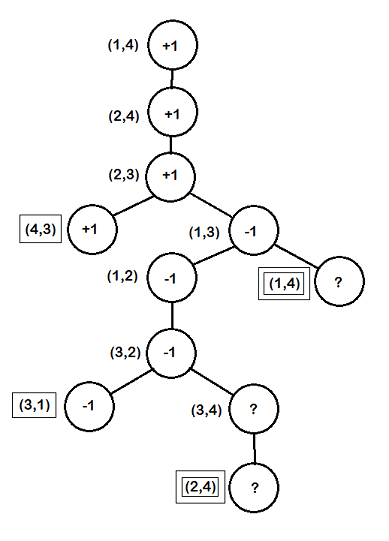
\includegraphics[scale=0.65]{9.png}
	\label{fig:9}
	\subsection*{5.}
	To handle the ? values, the agent is assumed to always choose to win when presented with a choice between winning and entering a ? state. This is equivalent to: min(-1, ?) = -1 and 		max(+1, ?) = +1. In the case that all possible choices are ?, then the backed-up value is ?.\newline
\end{document}